\documentclass{unizarpractice}
\usepackage[spanish,es-noquoting]{babel}
\usepackage[utf8x]{inputenc}
\usepackage{ucs}
\usepackage{lmodern}
\usepackage{tikz}
\usepackage{hyperref}
\usepackage{enumitem}

\usepackage{graphicx}

%\usetikzlibrary{arrows, shapes.misc}
\usepackage{float}
\usetikzlibrary{positioning, fit, calc, shapes, arrows}
\usepackage[underline=false]{pgf-umlsd}

\subject{Sistemas Distribuidos - 21/22}
\author{Unai Arronategui}
\title{Práctica 5: Raft 2ª parte}
\runningtitle{Práctica 5: Raft 2ª parte}

%\tikzset{
%    event/.style={circle, draw=black, fill=white, thin, minimum size=3mm},
%    event_ack/.style={event, fill=red!20},
%    event_req/.style={event, fill=green!20},
%    procnum/.style={rectangle, fill=white, inner sep=2mm},
%    mcmsg/.style={rectangle, draw=black, fill=blue!20, thin, minimum size=4.5mm},
%    request/.style={thick, green!40!black, -stealth'},
%    ack/.style={thick, red, -stealth'},
%    mc/.style={thick, blue, -stealth'},
%}

\begin{document}

\maketitle


\section*{Resumen}

En la práctica 5, se plantea construir un servicio de almacenamiento clave/valor, en memoria RAM, tolerante a fallos utilizando replicación distribuida basada en Raft, una solución de máquina de estados replicada mediante un algoritmo de consenso. Llamada rpc raft.SometerOperacion al lider distribuye la operacion, al resto de répics, mediante invocaciones RPC \textit{AppendEntries}. Las referencias son el tema 8 de teoría y el documento adjunto al guión. La especificación de estado de las reṕlicas y las llamadas RPC de referencia se encuentran disponibles en el anexo al final de este mismo guión.

\textbf{Estas prácticas incluyen redactar una memoria, escribir código fuente y elaborar un juego de pruebas. El texto de la memoria  y el código deben ser originales. Copiar supone un cero en la nota de prácticas.}


\subsection*{Notas sobre esta práctica}
\begin{itemize}
    \item Aplicar “go fmt” al código fuente. Además : fijar en el editor \textbf{máxima longitud de línea de 80 columnas, como mucho 20 instrucciones en una función} (salvo situaciones especiales justificadas). Existen diferentes posibilidades de editores con coloración sintáctica, acceso a efinición de tipos variables y funciones, etc:  vscode, gedit, geany, sublimetext, gvim, vim, emacs ...
    \item La solución aportada deberá funcionar para diferentes pruebas.
\end{itemize}


\setlength{\parskip}{\baselineskip}
\section{Objetivo de la práctica}

\noindent Los objetivos de la práctica son los siguientes:
\begin{itemize}[topsep=-0.5\baselineskip]
   \item Presentar  una implementación del algoritmo de eleccion de líder de Raft completo que funcione en escenarios  de fallos variados.
   \item Implementar el tratamiento de la llamada de RPC \textit{AppendEntry}, suponiendo un funcionamiento CON fallos.

\end{itemize}

\section{Eleccion de lider completa y llamada RPC \textit{AppendEntries} con fallos}

Se plantea implementar la solución completa de elección de ĺíder, incluida la restricción de nº de mandato y nº de índice para seleccionar al mejor líder (sección 5.4.1 del documento asociado), y la operativa de llamada RPC \textit{SometerOperacion} por parte de los clientes del sistema replicado que provocará llamadas \textit{AppendEntries} desde el lider a los seguidores con avance del indice de entradas de registro comprometidas. Ambos se desarrollarán en diferentes escenarios de fallos. Además se aplicará las operaciones sobre una máquina de estados simple, con operaciones de lectura y escritura sobre un almacen de datos en RAM mediante un tipo de datos \textit{map} de Golang.

\subsection{Funcionamiento}

Aunque es el lider el único que inicia la operativa de añadir nuevas entradas en el registro, todas las replicas tienen que enviar, de forma independiente, las operaciones comprometidas al servicio local de almacenamiento (máquina de estados) a través del canal de aplicación de operación. Mantaner ambas actividades bien separadas y tener cuidado de no incurrir en problemas de exclusión mutua.

\section{Organización de código}

Se aconseja el desarrollo del código y las pruebas en un ordenador Unix (Linux, BSDs, Mac, subsistema Linux de Windows). No se da soporte a desarrollo en Windows.

Implementar la funcionalidad de Raft, como algoritmo de consenso, en el fichero "raft/internal/raft/raft.go", donde ya disponeis de un esqueleto.

El conjunto del código reside en el \textit{modulo raft}, bajo el cual encontrais diferentes paquetes y funcionalidades, en subdirectorios. El subdirectorio ''\textit{raft/cmd}''  es utilizado par ubicar código ejecutable (func main). El subdirectorio ''\textit{raft/internal}'' se utiliza para paquetes de uso interno al modulo. En el subdirectorio ''\textit{raft/pkg}'' se ubican paquetes a exportar, que pueden ser utilizados por cógio externo al modulo. Y el subdirectorio ''\textit{raft/vendor}'' contiene los paquetes importados por el código de este modulo, y es obtenido ejecutando ''\textbf{go mod vendor}'' en el directorio raíz del modulo.

La implementación del servicio Raft de consenso debe ofrecer el siguiente interfaz de llamadas y tipo dato:

\begin{verbatim}
	// Crear nuevo nodo Raft
	nr:= NuevoNodo(nodos, yo, canalAplicar)
	
	// Someter operación para acuerdo por consenso en entrada de registro
	nr.SometerOperacion(operacion Operacion) (indice, mandato, esLider, idLider, valorADevolver)
	
	// Obtención de estado de nodo Raft: quien es, mandato en curso
	//y si cree ser el lider
	nr.ObtenerEstado() (yo, mandato, esLider, idLider)
	
	// Metodo Para() utilizado cuando no se necesita mas al nodo
	func (nr *NodoRaft) Para()
	
	// cada vez que una nueva operacion es comprometida en una entrada
	// de registro, cada nodo Raft debe enviar un mensaje AplicaOperacion
	// a la máquina de estados
	type AplicaOperacion	
\end{verbatim}

Teneis disponible la función "\textit{CallTimeout}", de llamada a método remoto rpc con tiempo de expiración, en el fichero "\textit{raft/internal/comun/rpctimeout}". Se ha actualizado con nueva versión que abre y cierra las conexiones TCP para cada llamada.

Teneis un código básico de servidor rpc genérico (con tcp, no http) en fichero "cmd/srvraft/main.go" (ya operativo) para que lo adapteis al funcionamiento de servidor Raft con registro de llamadas rpc \textit{AppendEntries} y \textit{RequestVote} desarrolladas en el fichero "\textit{internal/raft.raft.go}". \textbf{En est fichero, además se especifica un TipoOperador nuevo que dispone, como únicas operaciones posibles, las operaciones de lectura (operación ''leer'') y escritura (operación ''escribir'') a comprometer y aplicar a la máquina de estados que puede consistir en un almacen de datos implementado en GO con un tipo \textit{map[string]string}.}

Teneis disponible código de despliegue de programas remotos con ssh en multiples máquinas en el fichero "\textit{raft/internal/despliegue/sshClientWithPUBLICKEYAuthAndRemoteExec.go}".

Teneis disponible código incompleto, pero ejecutable, de test de integración para las 3 pruebas de validación en el fichero "\textit{raft/internal/testintegracionraft1/testintegracionraft1.go}". Incluye la primera prueba de la práctica 4, ya operativa. Para utilizarlo :

\begin{itemize}[topsep=-0.5\baselineskip]
	\item Generar pareja publica privada con algoritmo id\_ed25519 (ssh-keygen -t id\_ed25519), hacer una copia de seguridad del authorized\_keys antiguo, vaciar el authorized\_keys y copiar la nueva publica id\_ed25519.pub al authorized\_keys vacio. Comprobar con conexión ssh manual sin contraseña.
	\item Ubicar el modulo completo raft en el directorio \$HOME/tmp/p5/.
	\item cd a \$HOME/tmp/p4/raft y ejecutar go test -v internal/testintegracionraft1/	
\end{itemize}

Los datos de tipo de algoritmo de cifrado ssh y directorio de ubicación del modulo pueden ser modificados en este mismo fichero, si se ve más conveniente.

Los nombres de directorios, en el camino de acceso a vuestro código Golang, no deben contener el carácter espacio ni otros caracteres que dificulten el acceso a los ficheros fuente para la ejecución de procesos remotos.


\subsection{Validación}
La mayor parte del desarrollo, se puede trabajar en la máquina local, pero para la validación final debe ejecutarse cada servidor en una máquina física diferente. Comprobar, previamente y con tiempo suficiente, que no hay problemas en ejecución distribuida.

\noindent Se plantean las siguientes \textbf{pruebas a superar} y desarrollar test especificos para cada una de ellas :

\begin{enumerate}[topsep=-0.5\baselineskip]
\item Se consigue acuerdos de varias entradas de registro	a pesar de que un replica (de un grupo Raft de 3) se desconecta del grupo
\item NO se consigue acuerdo de varias entradas al desconectarse 2 nodos Raft de 3.	
\item Someter 5 operaciones cliente de forma concurrente y comprobar avance de indice del registro.

\end{enumerate}

Teneis ejemplos de tests incompletos en el fichero "\textit{internal/raft/integracionraft1.go}".

Para ejecutar todos los tests del modulo podeis ejecutar "\textit{go test  ./...}" en el diretorio raiz del modulo. Hay disponibles tambien métodos para ejecutar tests especificos. El comando "go test -v ./..." os permite tener más salida de información de depuración en la ejecución de tests completos de un modulo.


\section{Evaluación}
La realización de las prácticas es por parejas, pero los dos componentes de la pareja  \emph{deberán entregarla de forma individual}. En general, estos son los criterios de evaluación:
\begin{itemize}[topsep=-0.5\baselineskip]
\item Deben entregarse todos los programas, se valorará de forma negativa que falte algún programa / alguna funcionalidad.
\item Los programas no tendrán problemas de compilación, se valorará de forma muy negativa que no compile algún programa. 
\item Todos los programas deben funcionar correctamente como se especifica en el problema través de la ejecución de la bateria de pruebas.
\item Todos los programas tienen que seguir la guía de estilo de codificación de go fmt.
\item Se valorará negativamente una inadecuada estructuración de la memoria, así como la inclusión de errores gramáticales u ortográficos.
\item La memoria debería incluir diagramas de máquina de estados y diagramas de secuencia para explicar los \textbf{protocolos de intercambio de mensajes y los eventos de fallo}.
\item \textbf{Cada nodo}(servidor) \textbf{debe ejecutarse en una máquina física diferente en la prueba de evaluación}.
\end{itemize}

La superación de las prueba 1 supone la obtención de una B.  Para obtener una calificación de A, se deberá superar la prueba 1 y 2. La superación de los test 1, 2 y 3 supone tener una calificación de A+. Para llevar a cabo esta implementación, podeis basaros en el código disponible en el esqueleto.

%\begin{code}
%%% AUTOR: nombre y apellidos
%%% NIA: n'umero de identificaci'on del alumno
%%% FICHERO: nombre del fichero
%%% TIEMPO: tiempo en horas de codificaci'on
%%% DESCRIPCI'ON: breve descripci'on del contenido del fichero
%
%\end{code}
\subsection{Rúbrica}
Con el objetivo de que, tanto los profesores como los estudiantes de esta asignatura por igual, puedan tener unos criterios de evaluación objetivos y justos, se propone la siguiente rúbrica en el Cuadro~\ref{rubrica}. Los valores de las celdas son los valores mínimos que hay que alcanzar para conseguir la calificación correspondiente y tienen el siguiente significado:

\begin{itemize}[topsep=-0.5\baselineskip]
\item A+ (excelente). En el caso de software, conoce y utiliza de forma autónoma y correcta las herramientas, instrumentos y aplicativos software necesarios para el desarrollo de la práctica. Plantea \emph{correctamente} el problema a partir del enunciado propuesto e identifica las opciones para su resolución. Aplica el método de resolución adecuado e identifica la corrección de la solución, \emph{sin errores}. En el caso de la memoria, se valorará
una estructura y una presentación adecuadas, la corrección del lenguaje así como el contenido explica de forma precisa  los conceptos involucrados en la práctica.
En el caso del código, este se ajusta exactamente a las guías de estilo propuestas. 

\item A (bueno). En el caso de software, conoce y utiliza de forma autónoma y correcta las herramientas, instrumentos y aplicativos software necesarios para el desarrollo de la práctica. Plantea \emph{correctamente} el problema a partir del enunciado propuesto e identifica las opciones para su resolución. Aplica el método de resolución adecuado e identifica la corrección de la solución, \emph{con ciertos errores} no graves. Por ejemplo, algunos pequeños casos (marginales) no se contemplan o no funionan correctamente.
En el caso del código, este se ajusta \emph{casi} exactamente a las guías de estilo propuestas. 

\item B (suficiente). En el caso de software, conoce y utiliza de forma autónoma y correcta las herramientas, instrumentos y aplicativos software necesarios para el desarrollo de la práctica. No plantea correctamente el problema a partir del enunciado propuesto y/o no identifica las opciones para su resolución. No aplica el método de resolución adecuado y / o identifica la corrección de la solución, pero \emph{con errores}. En el caso de la memoria, bien
la estructura y / o la presentación son mejorables, el lenguaje presenta deficiencias y / o el contenido no explica de forma precisa los conceptos importantes involucrados en la práctica. En el caso del código, este se ajusta a las guías de estilo propuestas, pero es mejorable.

\item B- (suficiente, con deficiencias). En el caso de software, conoce y utiliza de forma autónoma y correcta las herramientas, instrumentos y aplicativos software necesarios para el desarrollo de la práctica. No plantea correctamente el problema a partir del enunciado propuesto y/o no identifica las opciones para su resolución. No se aplica el método de resolución adecuado y/o se identifica la corrección de la solución, pero \emph{con errores} de cierta gravedad y/o sin proporcionar una solución completa. 
En el caso de la memoria, bien
la estructura y / o la presentación son \emph{manifiestamente} mejorables, el lenguaje presenta \emph{serias} deficiencias y / o el contenido no explica de forma precisa los conceptos importantes involucrados en la práctica.
En el caso del código, hay que mejorarlo para que se ajuste a las guías de estilo propuestas.

\item C (deficiente). El software no compila o presenta errores graves. La memoria no presenta una estructura coherente y/o el lenguaje utilizado es pobre y/o contiene errores gramaticales y/o ortográficos. En el caso del código, este no se ajusta exactamente a las guías de estilo propuestas.
\end{itemize}

\begin{table}[h]
\centering
\begin{tabular}{|c|c|c|c|c|}
\hline
Calificación                   & Sistema & Tests & Código & Memoria \\ \hline
10                             & A+        & A+ (test 1-9)      & A+                          & A+                           \\ \hline
9                              & A+        & A+ (test 1-9)      & A                           & A                            \\ \hline
8                              & A        & A  (test 1-7)     & A                           & A                            \\ \hline
7                              & A         & A (test 1-7)       & B                           & B                            \\ \hline
6                              & B         & B (test 1-5)       & B                           & B                            \\ \hline
5                              & B-         & B-(test 1-4)        & B-                          & B-                           \\ \hline
\multicolumn{1}{|l|}{suspenso} & \multicolumn{4}{c|}{1 C}                                                          \\ \hline
\end{tabular}
\caption{Detalle de la rúbrica: los valores denotan valores mínimos que al menos se deben alcanzar para obtener la calificación correspondiente}
\label{rubrica}
\end{table}


\section{Entrega y evaluación}

\emph{Cada alumno} debe entregar un solo fichero en formato tar.gz o zip, a través de moodle en la actividad habilitada a tal efecto, \textbf{no más tarde del día anterior} a la siguiente sesión de prácticas (b5).

La entrega DEBE contener los diferentes ficheros de código Golang y la memoria (con un máximo de 6 páginas la memoria principal y 10 más para anexos), en formato pdf. El \textbf{nombre del fichero tar.gz debe indicar apellidos del alumno y nº de práctica}.  Aquellos alumnos que no entreguen la práctica no serán calificados. La evaluación “in  situ”  de  la práctica se realizará a partir de la sesión 6 de prácticas, incluida, hasta la semana de evaluación continua disponible en enero.
\begin{figure}
	\centering
	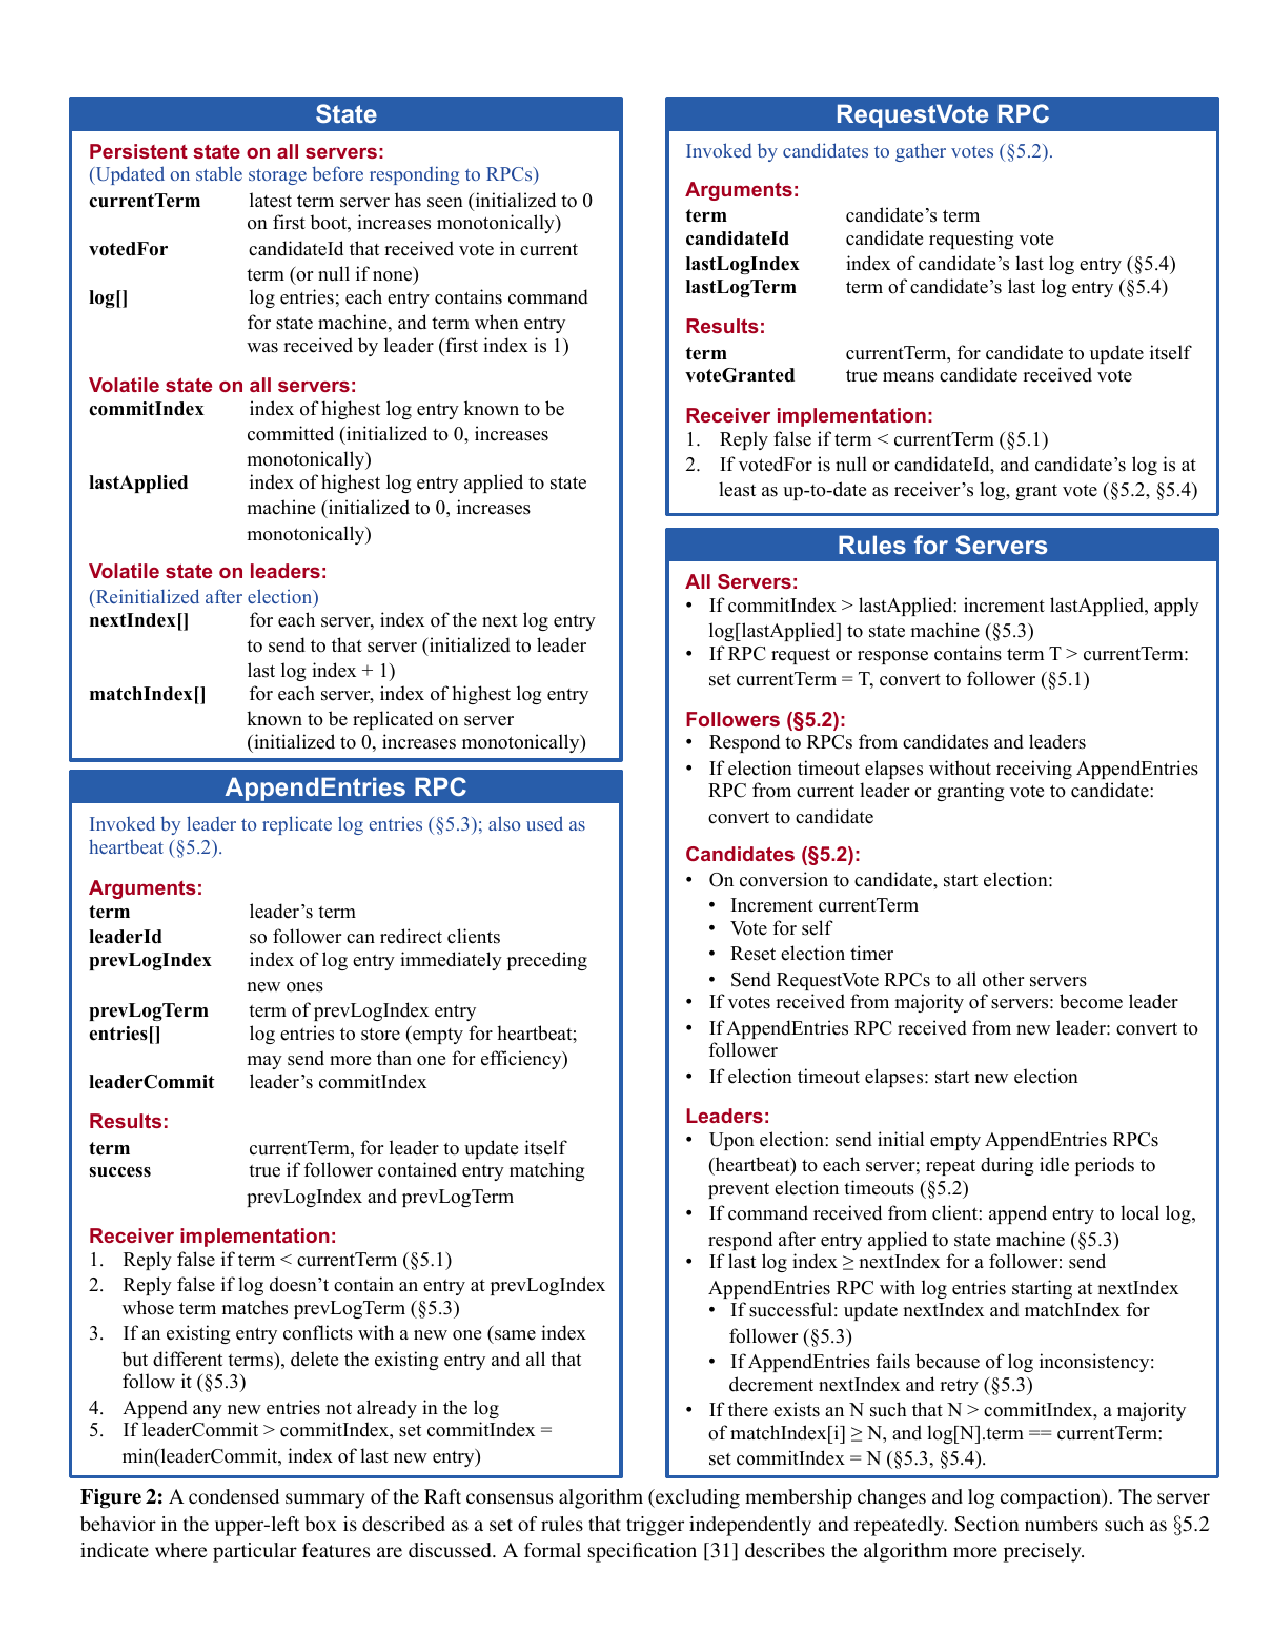
\includegraphics[width=1.15\linewidth]{RaftExtendedPaperSummary}
%%	\caption{Figura 2}
	\label{fig:raftextendedpapersummary}
\end{figure}


\end{document}
